\subsection{Attitude Controller}
The attitude controller for the quadcopter has been designed using a state space representation of the system. This helps handling the coupled angular response of the quadcopter. The chosen states for the system are the three angular positions and the three angular velocities. The input vector of the attitude system consists of the four motor rotational speeds and the output vector consists of the three angles, roll, pitch and yaw. Below, the state, input and the output vectors are presented.
%
\begin{flalign}
	\vec{x}(t) = 
	\begin{bmatrix}
		\phi & \theta & \psi & \dot{\phi} &	\dot{\theta} & \dot{\psi} \\
	\end{bmatrix}	\nonumber
	^T
	\label{xVector}
\end{flalign}  
\begin{flalign}
	\vec{y}(t) = 
	\begin{bmatrix}
		\phi &	\theta & \psi \\
	\end{bmatrix}	\nonumber
	^T
	\label{yVector}
\end{flalign}
\begin{flalign}
	\vec{u}(t)= 
	\begin{bmatrix}
		\omega_1 & \omega_2 &	\omega_3 &	\omega_4 \\
	\end{bmatrix}\nonumber	
	^T
	\label{uVector}
\end{flalign}
%
The above is then used in construction of the state space matrix representation as displayed in Equation \ref{xDotSS} and \ref{ySS}.
\begin{flalign}
	\vec{\dot{x}}(t)&=\vec{A} \cdot \vec{x}(t) + \vec{B} \cdot \vec{u}(t)
	\label{xDotSS} 
\end{flalign}
\begin{flalign}
	\vec{y}(t)&=\vec{C} \cdot \vec{x}(t) + \vec{D} \cdot \vec{u}(t)\label{ySS} 
\end{flalign}
\begin{where}
  \va{\vec{A}}{is the system matrix}{}
  \va{\vec{B}}{is the input matrix}{}
  \va{\vec{C}}{is the output matrix}{}
  \va{\vec{D}}{is the feed forward matrix}{}
\end{where}
The values for the A, B, C and D matrices are obtained from the linearized attitude equations, yielding the matrices shown below. As D is a zero matrix, only A, B and C are shown.
\footnotesize
\begin{flalign}   \label{Amatrix}
	\vec{A}=
	\begin{bmatrix}
		\ 0 & 0 & 0 & 1 & 0 & 0     \ \ \ \\ 
		\ 0 & 0 & 0 & 0 & 1 & 0     \ \ \ \\ 
		\ 0 & 0 & 0 & 0 & 0 & 1     \ \ \ \\
		\ 0 & 0 & 0 & 0 & 0 & 0     \ \ \ \\ 
		\ 0 & 0 & 0 & 0 & 0 & 0     \ \ \ \\ 
		\ 0 & 0 & 0 & 0 & 0 & 0     \ \ \  		
	\end{bmatrix}\nonumber
\end{flalign} \label{Bmatrix}
\begin{flalign}
    \vec{B} =
	\begin{bmatrix}
		\ 0 & 0 & 0 & 0      \ \ \ \\ 
		\ 0 & 0 & 0 & 0      \ \ \ \\ 
		\ 0 & 0 & 0 & 0      \ \ \ \\
		\ 0 & \si{-\frac{2 \cdot k_{th} \cdot L \cdot \overline{\omega}_2}{J_x}} & 0 & \si{\frac{2 \cdot k_{th} \cdot L \cdot \overline{\omega}_4}{J_x}}      \ \ \ \\ 
		\ \si{\frac{2 \cdot k_{th} \cdot L \cdot \overline{\omega}_1}{J_y}} & 0 & \si{-\frac{2 \cdot k_{th} \cdot L \cdot \overline{\omega}_3}{J_y}} & 0      \ \ \ \\ 
		\ \frac{2 \cdot k_d \cdot {\overline{\omega}_1}}{J_z} & - \frac{2 \cdot k_d \cdot {\overline{\omega}_2}}{J_z} & \frac{2 \cdot k_d \cdot {\overline{\omega}_3}}{J_z} & - \frac{2 \cdot k_d \cdot {\overline{\omega}_4}}{J_z}      \ \ \ 		
	\end{bmatrix}\nonumber
\end{flalign}
\begin{flalign} \label{Cmatrix}
	\vec{C} =	 
	\begin{bmatrix}
		\ 1 & 0 & 0 & 0 & 0 & 0     \ \ \ \\ 
		\ 0 & 1 & 0 & 0 & 0 & 0     \ \ \ \\ 
		\ 0 & 0 & 1 & 0 & 0 & 0     \ \ \ 		
	\end{bmatrix}\nonumber
\end{flalign}
\normalsize
%The designed attitude controller is depicted in the block diagram shown in Figure \ref{attitudeControlDiagram}.
%\begin{figure}[H]
%	\centering
%	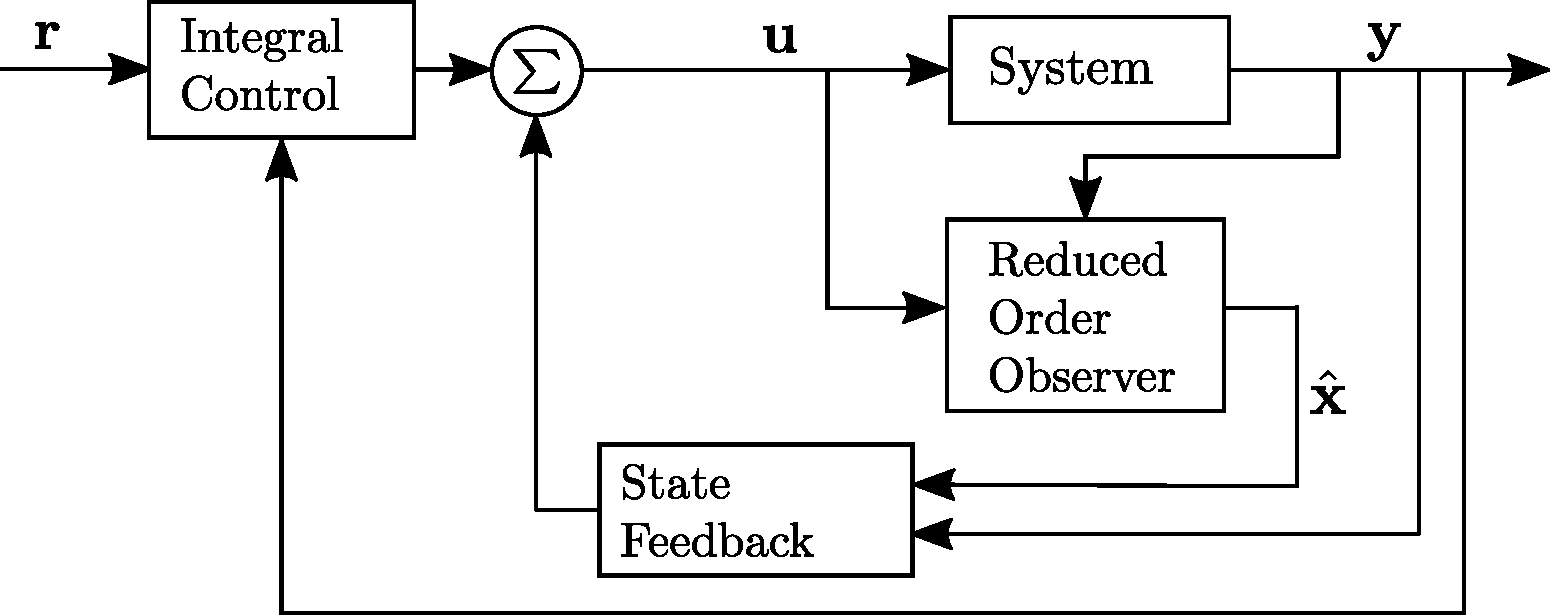
\includegraphics[scale=0.3]{figures/AttitudeControlDiagram}
%	\caption{Control structure for regulating the attitude response of the quadcopter. It includes the state feedback, the reduced order observer and the integral term.}
%	\label{attitudeControlDiagram}
%\end{figure}

State feedback and integral control
For the quadcopter to hover, it is desired to keep the attitude in equilibrium; this is achieved using a state feedback. To be able to change and track a reference an integral controller is designed around the state feedback. This allows changing the attitude in order to move in the xy-plane of the inertial system.












